\documentclass{report}

\usepackage{listings}
\usepackage[vlined, boxed]{algorithm2e}
\usepackage{tikz}
\usepackage{hyperref}
\usepackage{float}
%\usepackage{geometry}
\usepackage{mathtools}
\usepackage{amssymb}
\usepackage{galois}
\usepackage{titlesec}
\usepackage{stmaryrd}
\usepackage{tabularx}
\usepackage{fancyvrb}
\usepackage{enumitem}
\usepackage{breakcites}
\usepackage{listings}
\usepackage{xcolor}
\usepackage{adjustbox}




\titleformat{\chapter}[hang]
  {\normalfont\huge\bfseries}   % formatting for chapter title (font size, style)
  {\thechapter.}                % the label (chapter number followed by a period)
  {1em}                         
  {}
\titlespacing*{\chapter}{0pt}{0pt}{20pt}

\SetAlCapSkip{2mm}

\newcommand\nElement{\mathrlap{\perp}\top}

\title{\Huge{}Implementation and Evaluation of~the FunArray\\[1em]\large{}Bachelor's Thesis\\[1em]Software and Computational Systems Lab\\Ludwig-Maximilians-Universit\"at M\"unchen}
\date{October 2024}
\author{Maximilian Hofstetter}

\newcommand{\funArray}[1]{$#1$}
\newcommand{\bound}[1]{\{#1\}}
\newcommand{\fvalue}[1]{\;#1\;}



\begin{document}

\maketitle

\section*{Statement of Originality}
\thispagestyle{empty}
I hereby confirm that I have written the accompanying thesis by myself, without contributions from any sources other than those cited in the text and acknowledgements. This applies also to all graphics, drawings and images included in the thesis.

\section*{Utilised Aids in Creating this Thesis}

I did not rely any LLM to produce any text in this thesis, nor any other tool automatically generating text. For writing program code i took advantage of IDE features such as auto-completion. This in parts includes the IntelliJ IDEA full line completion\footnote{\url{https://www.jetbrains.com/help/idea/full-line-code-completion.html}}, which is an auto-complete tool relying on a locally run deep learning model. It is not able to suggest any in-depth design choices or code fragments that exceed the scope of a single line.

\section*{Attachments}

The following attachments have been submitted together with this thesis via Uni2Work:

\begin{enumerate}
	\item Java source code for my implementation of the FunArray and the static Analyser
	\item Utilised SV-Comp benchmarks in the C language
	\item Utilised SV-Comp benchmarks translated into the embedded domain specific language
	\item Generated output when executing the provided benchmarks
\end{enumerate}

\section*{Acknowledgements}

I would like to express my gratitude to my thesis advisor Gidon Ernst for extensively supporting me throughout the implementation and writing process of this thesis and for translating the utilised benchmarks into a EDSL.


\setcounter{tocdepth}{1}
\tableofcontents

\chapter{Introduction}


%Verifikation ist wichtig
%
%Arrays sind schwierig
%
%Es gibt das von Cousot


Dividing any scalar value by zero is undefined behaviour in most programming languages and will certainly throw an error. When an experienced programmer is writing code, they make sure to include checks to rule out this behaviour. But when code becomes more complex, it is often times not that easy to manually detect when a division by zero might occur. It is therefore common to analyse code automatically to detect problems of this kind. Consider the following program written in Java:


\begin{center}
\begin{BVerbatim}
class Main {
  public static void main(String[] args) {
    int result = 1 / 0;
    System.out.println(result);
  }
}
\end{BVerbatim}
\end{center}

\noindent To a human observer it is immediately obvious that this snippet contains a division by zero and will result in some undesired behaviour. When executing this code snippet, the JVM will output the following error message: \texttt{Exception in thread "main" java.lang.ArithmeticException: Division by zero}. But even when only writing this faulty piece of code, without having actually executed it, our IDE will issue a warning: \texttt{Division by zero}. Apparently our IDE has some functionality built in that detects any such division by zero. How is this being accomplished? One immediate guess to this would be the assumption that it syntactically verifies that the code does not contain the string \texttt{/0} anywhere. Let us modify our snippet to check this hypothesis:

 \begin{center}
\begin{BVerbatim}
class Main {
  public static void main(String[] args) {
    int divisor = 458;
    divisor = divisor + 17;
    divisor = divisor - 475;
    int result = 1 / divisor;
    System.out.println(result);
  }
}
\end{BVerbatim}
\end{center}

\noindent The code is now obfuscated in such a way that a human code reviewer might not notice the division by zero on first glance. Any syntactic analysis should also be impossible. However our IDE still issues a warning: \texttt{Division by zero}. This process of analysing code without actually reviewing it, is called static analysis. This term summarises a lot of different techniques, one of which is abstract interpretation.
To put it very simple, when doing abstract interpretation, we are not running the program on concrete values, but rather on their properties. Let us take a look our example but this time with comments on what we can conclude by only taking the scalar variables sign property into account.  


\lstset{
    basicstyle=\ttfamily,
    commentstyle=\color{gray},  % Set the color of comments
    morecomment=[l]{//},        % Define "//" as the start of a comment
}
\vspace{2mm}

\begin{adjustbox}{center}
\begin{lstlisting}
class Main {
  public static void main(String[] args) {
    int divisor = 458;
    // divisor references a positive integer
    divisor = divisor + 17;
    // when adding to positive numbers the result
    // will also be positive. the value of the 
    // variable divisor must still be positive
    divisor = divisor - 475;
    // when subtracting from a positive number,
    // the result might be negative or zero
    // the variable divisor might potentially
    // be zero
    int result = 1 / divisor;
    // since divisor might be zero, this division 
    // might potentially throw an error!
    System.out.println(result);
  }
}
\end{lstlisting}
\end{adjustbox}
\vspace{2mm}

\noindent Without having concretely calculated every step of the program, we have arrived at the conclusion that there may potentially be a division by zero. What we have done in natural language, can also be done in a formal way that is easily automated \cite{cousot1977} as long as only scalar variables are present. Now let us review an example that not only includes scalar variables but also arrays.


\vspace{2mm}

\begin{adjustbox}{center}
\begin{lstlisting}
class Main {
  public static void main(String[] args) {
    int[] array = new int[10];
    for (int i = 10; i > 0; i--) {
      array[i] = i;
    }
    for (int j : array) {
      System.out.println(1 / j);
    }
  }
}
\end{lstlisting}
\end{adjustbox}
\vspace{2mm}


\noindent Once again we would like to make sure that no division by zero occurs. On first sight it seems as if this was the case, but there is actually a off-by-one error hidden in the first loop and the array element at the first index will actually be a zero.
How can we check for mistakes like these without executing the program? Of course we would be able to keep track of every property of every element on its own. However, this becomes problematic as soon as an array's length is being determined at runtime and when running it in the abstract, only certain properties are known about the length. The solution to this is the FunArray \cite{cousot2011}. It is a technique where an array is divided into symbolic segments and properties are being determined for these segments. Consider figure~\ref{fig:funarray}. It shows a graphical representation of a FunArray, that has two segments, which contain only positive and negative elements respectively. The shared bound in the middle is determined by the variable value of \texttt{i}, which itself is an abstract value. The length of the array and therefore the right bound of the second segment is also determined by an abstract value \texttt{l} and does not necessitate calculating the length in the concrete.

\begin{figure}[!htb]
\vspace{0.2cm}
\begin{center}
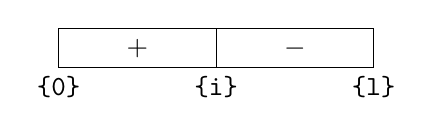
\begin{tikzpicture}
	\draw (0,0) -- (4,0);
    \draw (0,0.5) -- (4,0.5);

    \draw (0,0) -- (0,0.5);
    \draw (0,-0.25) node {\texttt{\string{0\string}}};

    \draw (1,-0.05) node[anchor=south, yshift=0.5mm] {$+$};

    \draw (2,0) -- (2,0.5);
    \draw (2,-0.25) node {\texttt{\string{i\string}}};
    
    \draw (3,0) node[anchor=south] {$-$};
    
    \draw (4,0) -- (4,0.5);
    \draw (4,-0.25) node {\texttt{\string{l\string}}};
\end{tikzpicture}
\end{center}
\caption{A graphical representation of a FunArray.} \label{fig:funarray}

\end{figure}

\noindent The FunArray technique advances the field of abstract interpretation as it is an automatic way to semantically infer segments on arrays. It can easily be introduced to existing analyses without having any significant impact on execution time. It also does not require any additional effort by programmers as it is fully-automatic and it can be combined with any arbitrary abstract domain. In this thesis I will show how I implemented an abstract analyser that utilises the FunArray. I will then test it on a selection of Benchmarks and determine how many of the included assertion obligations can automatically be proven with this approach and how often the analyser at least determines non-trivial invariants for any loops present.



Goal: To implement the FunArray and evaluate it on practical benchmarks

Was kann die Implementierung (Contribution)

Referenzen zu einzelnen Kapiteln (Ich hab so und so viele Invarianten gefunden)

Konkrete Zahlen direkt reinpacken


Array Smashing ist deswegen schlechter, weil die Invarianten mehr als ein

Zeigen dass man nicht-triviale Invarianten hat, aber 


Vielleicht kann man Limitierung DNF umgehen indem man weniger joined und Fallunterscheidungen macht




















 
\chapter{Background} \label{chap:background}





\section{Properties}

Consider a set of entities $\mathcal{E}$. A formal property $P\subseteq \wp(\mathcal{E}) $ is a set of entities that have this property \cite[chapter 8]{cousot2021}. In the introduction we abstracted the value of a variable, that would be an integer in the concrete, to its sign. With the set of integers as our set of entities $\mathcal{E}=\mathbb{Z}$, a ``positive'' property is defined as $P_{pos}=\{z\in \mathcal{E} \;|\; 0<z\}$ and we can define some more semantic properties like in table \ref{table:properties}.
\begin{table}[hbt]
\begin{center}
  \begin{tabular}{l|l}
  $\mathsf{false}$ & $\emptyset$\\
   $P_{0}$ & $\{0\}$\\
   $P_{pos}$ & $\{z\in \mathbb{Z} \;|\; 0<z\}$\\
   $P_{neg}$ & $\{z\in \mathbb{Z} \;|\; 0>z\}$\\
   $P_{pos0}$ & $\{z\in \mathbb{Z} \;|\; 0\leq z\}$\\
   $P_{neg0}$ & $\{z\in \mathbb{Z} \;|\; 0\geq z\}$\\
   $P_{even}$ & $\{z\in \mathbb{Z} \;|\; \exists k\in\mathbb{Z}:2k=z \}$ \\
   $P_{odd}$ & $\{z\in \mathbb{Z} \;|\; \exists k\in\mathbb{Z}:2k+1=z \}$ \\
   $P_{pos\_even}$ & $\{z\in \mathbb{Z} \;|\; z>0 \wedge \exists k\in\mathbb{Z}:2k=z \} = P_{pos} \cap P_{even}$ \\
   $\vdots$ &$\vdots$\\
   $\mathsf{true}$ & $\mathbb{Z}$\\
  \end{tabular}
  \caption{An incomplete selection of properties for $\mathbb{Z}$.}\label{table:properties}
  \end{center}
\end{table}

\noindent We call a property $P$ ``stronger'' than $P'$ (or $P'$ ``weaker'' than $P$) if $P\subseteq P'$. Its set representation contains less elements and we therefore have more information about an element that fulfils said property. The weakest property is the $\mathsf{true}$ property that is satisfied by alle elements and the strongest is $\mathsf{false}$ which is satisfied by none \cite[chapter 8]{cousot2021}. Not all properties from $\wp(\mathcal{E})$ carry a semantic meaning. We therefore only consider the set of properties of interest $C\subseteq\wp(\mathcal{E})$. If we want to analyse the signs of integers this could be $C_{sign}=\{\mathsf{false}, P_{0}, P_{pos}, P_{neg}, P_{pos0}, P_{neg0}, P_{not0}, \mathsf{true}\}$. The poset  $\langle C,\subseteq\rangle$ is called the ``concrete domain''.

\section{Abstraction}\label{sec:abstraction}

Now consider a set of abstract properties $A$. This is not a power set of concrete values anymore but a set of purely semantic symbols that represent abstract properties. If there exists a Galois connection $\langle C,\subseteq\rangle \galois{\alpha}{\gamma}\langle A\sqsubseteq\rangle$, we call $\langle A\sqsubseteq\rangle$ the abstract domain, $\alpha\in C\to A$ the abstraction function and $\gamma\in A\to C$ the concretisation function \cite[chapter 11]{cousot2021}. To put the working principle of Galois connections into simple terms: $A$'s elements abstract $C$'s elements and $\sqsubseteq$ works analogous in the abstract to $\subseteq$ in the concrete. More formally: $\forall P_C\in C:\forall P_A \in A:\alpha(P_C)\sqsubseteq P_A \Longleftrightarrow P_C \subseteq \gamma(P_A)$.

\begin{figure}[htb]
	\begin{center}
		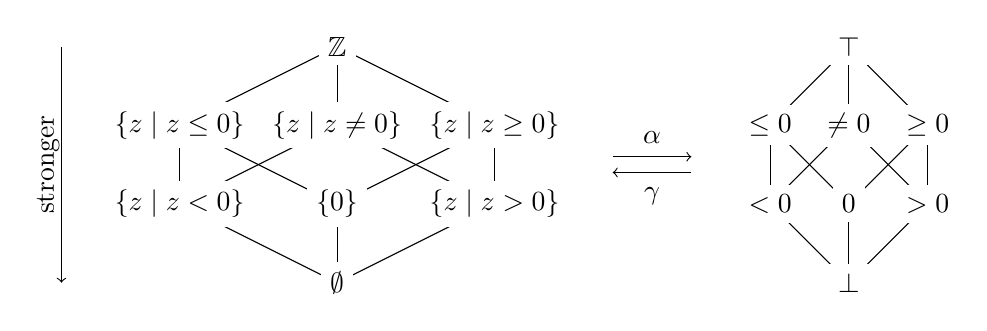
\begin{tikzpicture}
			% Concrete domain
			\draw (-4.5,0) -- (-6.5,1);
            \draw (-4.5,0) -- (-4.5,1);
            \draw (-4.5,0) -- (-2.5,1);
            \draw (-4.5,3) -- (-6.5,2);
            \draw (-4.5,3) -- (-4.5,2);
            \draw (-4.5,3) -- (-2.5,2);
            
            \draw (-4.5,1) -- (-6.5,2);
            \draw (-4.5,1) -- (-2.5,2);
            \draw (-6.5,1) -- (-6.5,2);
            \draw (-2.5,1) -- (-2.5,2);
            \draw (-4.5,2) -- (-6.5,1);
            \draw (-4.5,2) -- (-2.5,1);
            
            \draw (-4.5,0) node[fill=white!5] {$\emptyset$};
            \draw (-6.5,1) node[fill=white!5] {$\{z\;|\;z<0\}$};
            \draw (-4.5,1) node[fill=white!5] {$\{0\}$};
            \draw (-2.5,1) node[fill=white!5] {$\{z\;|\;z>0\}$};
            \draw (-6.5,2) node[fill=white!5] {$\{z\;|\;z\leq0\}$};
            \draw (-4.5,2) node[fill=white!5] {$\{z\;|\;z\neq0\}$};
            \draw (-2.5,2) node[fill=white!5] {$\{z\;|\;z\geq0\}$};
            \draw (-4.5,3) node[fill=white!5] {$\mathbb{Z}$};

			% Abstract domain
            \draw (2,0) -- (1,1);
            \draw (2,0) -- (2,1);
            \draw (2,0) -- (3,1);
            \draw (2,3) -- (1,2);
            \draw (2,3) -- (2,2);
            \draw (2,3) -- (3,2);
            
            \draw (2,1) -- (1,2);
            \draw (2,1) -- (3,2);
            \draw (1,1) -- (1,2);
            \draw (3,1) -- (3,2);
            \draw (2,2) -- (1,1);
            \draw (2,2) -- (3,1);
            
            \draw (2,0) node[fill=white!5] {$\perp$};
            \draw (1,1) node[fill=white!5] {$<0$};
            \draw (2,1) node[fill=white!5] {$0$};
            \draw (3,1) node[fill=white!5] {$>0$};
            \draw (1,2) node[fill=white!5] {$\leq0$};
            \draw (2,2) node[fill=white!5] {$\neq0$};
            \draw (3,2) node[fill=white!5] {$\geq0$};
            \draw (2,3) node[fill=white!5] {$\top$};
            
            
            % Arrows
            \draw (-0.5,1.85) node {$\alpha$};
            \draw [->](-1,1.6) -- (0,1.6);
            \draw [<-](-1,1.4) -- (0,1.4);
            \draw (-0.5,1.1) node {$\gamma$};
            
            \draw [<-](-8,0) -- (-8,3);
            \draw (-8.17,1.5) node[rotate=90] {stronger};
        \end{tikzpicture}
        \caption{The sign properties of the concrete integer domain (left) next to the abstract sign domain (right) as a Hasse diagram \cite{cousot2021}.}
	\end{center}
\end{figure}

\section{A Simple Language}

Consider a simple programming language as defined in figure \ref{fig:bnf_simplelanguage}. In the following sections we will assign it concrete semantics for actually executing a program written in this language in the concrete. We will then compare this concrete semantics to an abstract interpretation of the language.

\begin{figure}[!htb]
\begin{center}
\begin{tabular}{rcl}
	
program \texttt{p} $\in\mathbb{P}$& ::= & \texttt{A[e] := e}\\
  &$|$&  \texttt{x := e}\\
  &$|$&  \texttt{p$_\mathtt{1}$; p$_\mathtt{2}$}\\
  &$|$&  \texttt{if b then p$_\mathtt{1}$ else p$_\mathtt{2}$}\\
  &$|$&  \texttt{while b then p}\\
  \\
  boolean expression \texttt{b} $\in\mathbb{B}$ & ::= & \texttt{e$_\mathtt{1}$<e$_\mathtt{2}$} $|$  \texttt{e$_\mathtt{1}$<=e$_\mathtt{2}$} $|$ \texttt{!e} $|$ \texttt{e$_\mathtt{1}$==e$_\mathtt{2}$}\\
	\\
	arithmetic expression \texttt{e} $\in\mathbb{E}$ & ::= & \texttt{z} $|$ \texttt{x} $|$ \texttt{A[e]} $|$ \texttt{e$_\mathtt{1}$+e$_\mathtt{2}$} $|$ \texttt{e$_\mathtt{1}$-e$_\mathtt{2}$} $|$ \texttt{e$_\mathtt{1}$*e$_\mathtt{2}$} $|$ \texttt{e$_\mathtt{1}$/e$_\mathtt{2}$}\\

  \\
	numeral \texttt{z}&$\in$&$\mathbb{Z}$\\
	scalar variable name \texttt{x}&$\in$&$\mathbb{X}$\\
	array variable name \texttt{A}&$\in$&$\mathbb{A}$\\
\end{tabular}
\end{center}
\caption{The grammar for a simple example language in Backus--Naur form.}\label{fig:bnf_simplelanguage}
\end{figure}

\section{Expression Semantics}

Determining the meaning of a particular statement requires us to know the current state of the program. The expression \texttt{i + 1} has an entirely different result, depending on the value of the variable \texttt{i}, which is recorded in the program's concrete scalar variable environment. An environment is defined as a function $\rho\in\mathcal{R}_v$ with $\mathcal{R}_v \triangleq \mathbb{X}\mapsto\mathcal{V}$, where $\mathbb{X}$ is the set of syntactical variable names and $\mathcal{V}$ is the set of values they can take \cite{cousot2011}.
Now consider the simple syntactical expression $\mathtt{e}\in\mathbb{E}$. It only contains scalar constants, scalar variable references and operators. Now $\llbracket\mathtt{e}\rrbracket\rho$ describes the semantics of \texttt{e} in the concrete variable environment $\rho$. The semantics of a variable \texttt{i} is defined as $\llbracket\mathtt{i}\rrbracket\rho=\rho(\mathtt{i})$ and the semantics of a syntactic operator $\circledast$ is defined as $\llbracket\mathtt{e_0\circledast e_1}\rrbracket\rho=\llbracket\mathtt{e_0}\rrbracket\rho \ast\llbracket\mathtt{e_1}\rrbracket\rho$ \cite{scott1971}. 
Imagine a variable environment $\rho$, where $\rho(\mathtt{i})=1$, for example. Our previously mentioned expression \texttt{i + 1} evaluates to:

\begin{equation*}
\begin{aligned}
\llbracket\mathtt{i \;\texttt{+}\; 1}\rrbracket\rho &=\llbracket\mathtt{i}\rrbracket\rho +\llbracket\mathtt{1}\rrbracket\rho \\
& = \rho(\mathtt{i}) + 1\\
& = 1+1\\
& = 2
\end{aligned}
\end{equation*}
\vspace{1mm}

\noindent When executing programs in the abstract, we cannot rely on integer arithmetics to define our semantics. Instead we will have to define an abstract counterpart $f^\#$ for every concrete operator $f$. An abstract interpretation is consistent with the concrete execution, iff $f(x)\subseteq\gamma(f^\#(\alpha(x)))$, as shown in figure \ref{fig:abstractfunction} \cite{cousot1977}.

\begin{figure}[htb]
	\begin{center}
		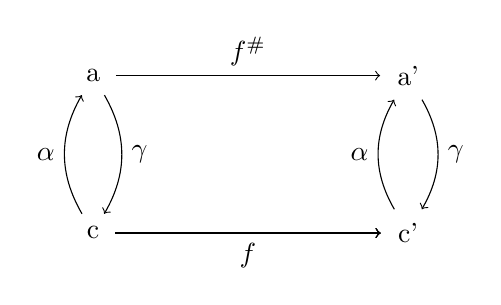
\begin{tikzpicture}
%            

         \node [circle] (A)  at (0,0)    {c};
  		 \node [circle] (B)  at (4,0)    {c'};
  		 \node [circle] (C)  at (0,2)    {a};
  		 \node [circle] (D)  at (4,2)    {a'};
  		 
  		 \draw [->] (A) --node[below]{$f$} (B); 
  		 \draw [->] (C) --node[above]{$f^\#$} (D); 
  		 \draw [->] (A) to [bend left=30] node[left]{$\alpha$}  (C); 
  		 \draw [->] (C) to [bend left=30] node[right]{$\gamma$} (A); 
  		 \draw [->] (B) to [bend left=30] node[left]{$\alpha$} (D); 
  		 \draw [->] (D) to [bend left=30] node[right]{$\gamma$} (B); 
  		 
  		 
  		 \draw [->] (A) -- (B); 
  		 \draw [->] (A) -- (B); 
  		 \draw [->] (A) -- (B); 
         
        \end{tikzpicture}
        \caption{The abstraction of a concrete function $f$.}\label{fig:abstractfunction}.
	\end{center}
\end{figure}

\noindent This ensures that the abstract result of an operation includes at least (but not necessarily only) the result that the operation would have in the concrete. Let us take a look at the multiplication operation \texttt{*}. Its concrete semantics $\llbracket\mathtt{e_1\texttt{ * } e_2}\rrbracket\rho$ is trivially defined as $\llbracket\mathtt{e_1}\rrbracket\rho \times\llbracket\mathtt{e_2}\rrbracket\rho$. When we want to interpret this operation in the abstract domain of signs $\llbracket\mathtt{e_1\texttt{ * } e_2}\rrbracket\rho$, we will now have to come up with a definition of sign multiplication $\times_\pm$. The most trivial of these would be $\llbracket\mathtt{e_1\texttt{ * } e_2}\rrbracket\rho=\top$, meaning the result is unknown. We can, however, further narrow down a more precise definition as can be seen in table \ref{table:multiply}. This satisfies our condition for an abstract operation, since $\times(x,y)\subseteq\gamma(\times_\pm(\alpha(x),\alpha(y)))$ for all $x,y\in\mathbb{Z}$ and it also makes intuitive sense, as for example a multiplication of two positive integers will result in another positive integer, a multiplication of any integer with zero will result in zero and so on.


\begin{table}[hbt]
\begin{center}
\begin{tabular}{c|c|c|c|c|c|c|c|c}
            $\times_\pm$& $\perp$ & $<0$    & $0$     & $>0$    & $\leq0$ & $\neq0$ & $\geq0$ & $\top$  \\ \hline
            $\perp$ & $\perp$ & $\perp$ & $\perp$ & $\perp$ & $\perp$ & $\perp$ & $\perp$ & $\perp$ \\
            $<0$    & $\perp$ & $>0$    & $0$     & $<0$    & $\geq0$ & $\neq0$ & $\leq0$ & $\top$  \\
            $0$     & $\perp$ & $0$     & $0$     & $0$     & $0$     & $0$     & $0$     & $0$     \\
            $>0$    & $\perp$ & $<0$    & $0$     & $>0$    & $\leq0$ & $\neq0$ & $\geq0$ & $\top$  \\
            $\leq0$ & $\perp$ & $\geq0$ & $0$     & $\leq0$ & $\geq0$ & $\top$  & $\leq0$ & $\top$  \\
            $\neq0$ & $\perp$ & $\neq0$ & $0$     & $\neq0$ & $\top$  & $\neq0$ & $\top$  & $\top$  \\
            $\geq0$ & $\perp$ & $\leq0$ & $0$     & $\geq0$ & $\leq0$ & $\top$  & $\geq0$ & $\top$  \\
            $\top$  & $\perp$ & $\top$  & $0$     & $\top$  & $\top$  & $\top$  & $\top$  & $\top$ 
        \end{tabular}
  \caption{A table showcasing the result of the abstract property transformer $\times_\pm$ which is an abstraction of the concrete multiplication operator.}\label{table:multiply}
  \end{center}
\end{table}

\section{Transformers}

Our simple language not only contains expressions, but also commands or statements that modify the environment itself. For example, consider the environment $\rho$ where $\rho(\mathtt{i})=1$. After executing the command \texttt{i := i + 1}, the value of the variable \texttt{i} changes and therefore the environment $\rho'$ after the execution of the command is different from $\rho$. We write $\llbracket \texttt{i\;:=\;i\;+\;1} \rrbracket\rho=\rho[\mathtt{i}:=\texttt{i\;+\;1}]=\rho'$, meaning the semantics of the environment $\rho$ after executing an assignment \texttt{i\;:=\;i\;+\;1} is an environment $\rho'$ where all occurrences of \texttt{i} have been replaced by \texttt{i\;+\;1}. 
More generally the semantics of an assignment is defined as $\llbracket \texttt{i\;:=\;e} \rrbracket\rho=\rho[\mathtt{i}:=\texttt{e}]$ with $\rho[\mathtt{i}:=\texttt{e}](\mathtt{i})=\llbracket\mathtt{e}\rrbracket\rho$ \cite{cousot2011}. Commands that alter the environment are called transformations. They are basically functions in $\mathcal{R}_v\mapsto\mathcal{R}_v$ \cite{scott1971}.
The process in an abstract interpretation is the same, with the difference being of course, that expressions are being evaluated in the abstract domain.

\section{Conditionals}\label{sec:conditionals}

The concrete semantics for conditionals is relatively obvious. Consider the statement $\texttt{if v}_\texttt{1}\texttt{<=v}_\texttt{2} \texttt{ then p}_\texttt{1} \texttt{ else p}_\texttt{2}$. We test whether the variable $\texttt{v}_\texttt{1}$ is less equal than $\texttt{v}_\texttt{2}$ and if that is the case we execute the program branch $\texttt{p}_\texttt{1}$ and $\texttt{p}_\texttt{2}$ otherwise. The semantics for this are defined as follows \cite{scott1971}: 

\begin{center}
	$\llbracket\texttt{if v}_\texttt{1}\texttt{<=v}_\texttt{2} \texttt{ then p}_\texttt{1} \texttt{ else p}_\texttt{2}\rrbracket\rho = 
	\begin{cases}
		\llbracket\texttt{p}_\texttt{1}\rrbracket\rho, & \textrm{if } \llbracket\texttt{v}_\texttt{1}\rrbracket\rho \leq \llbracket\texttt{v}_\texttt{2}\rrbracket\rho\\
		\llbracket\texttt{p}_\texttt{2}\rrbracket\rho, & \textrm{else}
	\end{cases}$
\end{center} 
\vspace{2mm}
\noindent The semantics in an abstract analyses work slightly different. Since $\texttt{v}_\texttt{1}$ and $\texttt{v}_\texttt{2}$ do not have concrete values, but are being abstracted by abstract values that might contain more than one value, we cannot always decide whether the condition is true or not. Instead we will have to calculate both branches and need to restrict the variable values in such a way that the condition is definitely true and definitely false respectively. The semantics in the abstract are as follows:

\begin{center}
	$\llbracket\texttt{if v}_\texttt{1}\texttt{<=v}_\texttt{2} \texttt{ then p}_\texttt{1} \texttt{ else p}_\texttt{2}\rrbracket\rho = \llbracket\texttt{p}_\texttt{1}\rrbracket\rho^{t\!t} \sqcup\llbracket\texttt{p}_\texttt{2}\rrbracket\rho^{f\!\!f}$,
\end{center} 

\noindent whereby $\rho^{t\!t}=\rho[v_1:=v_1'][v_2:=v_2']$ is such that $v_1'\sqsubseteq v_1$ and $v_2'\sqsubseteq v_2$ and $v_1'\leq v_2'$. Analogous for $\rho^{f\!\!f}$. How  $v_1'$ and $v_2'$ are determined depends on the used abstract domain.

\section{Fixpoint Analysis}\label{sec:fixpoint_analysis}

The semantics for loops in the concrete are defined recursively like follows \cite{scott1971}:

\begin{center}
	$\llbracket\texttt{while b do p}\rrbracket = 
	\begin{cases}
		\llbracket\texttt{p}\rrbracket \circ \llbracket\texttt{while b do p}\rrbracket, & \textrm{if } \llbracket\texttt{b}\rrbracket=\textrm{tt}\\
		\textrm{empty program}, & \textrm{else}
	\end{cases}$
\end{center} 
\vspace{2mm}

\noindent Once again we face the problem in abstract interpretation whether and when the condition \texttt{b} is satisfied. Instead we will relay on a technique called fixpoint analysis. Basically we satisfy the condition \texttt{b} and then apply the command \texttt{p} until we reach a fixpoint, meaning that the state $\rho$ does not change anymore when applying \texttt{p} \cite{cousot1977}. Let us regard the application of the program \texttt{p} as a function $f: \mathcal{R}_v\mapsto \mathcal{R}_v$. Now $\rho^0$ describes the variable environment before entering the loop, $\rho^n=f(\rho^{n-1})$ describes the environment after executing \texttt{p} $n$ times. When repeatedly executing $f$, we obtain a sequence that follows one of the three following patterns:

\begin{enumerate}
	\item A continuous sequence, where we reach a state that has not been obtained before after each loop pass.\\
\begin{center}
	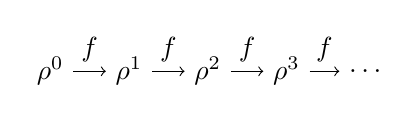
\begin{tikzpicture}
	\node (A) at (0,0) {$\rho^0$};
	\node (B) at (1,0) {$\rho^1$};
	\node (C) at (2,0) {$\rho^2$};
	\node (D) at (3,0) {$\rho^3$};
	\node (E) at (4,0) {$\ldots$};
	
	
	\draw[->] (A) -- node[above]{$f$} (B);
	\draw[->] (B) -- node[above]{$f$} (C);
	\draw[->] (C) -- node[above]{$f$} (D);
	\draw[->] (D) -- node[above]{$f$} (E);
\end{tikzpicture}
\end{center}

	\item \parbox[t]{\linewidth}{A sequence that ends in a cycle, meaning the sequence will repeat multiple states for ever.\\
\begin{center}
	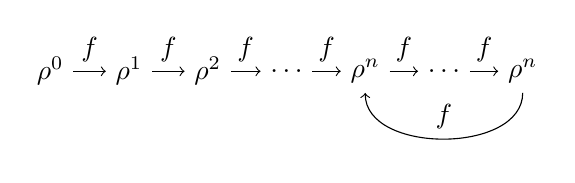
\begin{tikzpicture}
	\node (A) at (0,0) {$\rho^0$};
	\node (B) at (1,0) {$\rho^1$};
	\node (C) at (2,0) {$\rho^2$};
	\node (D) at (3,0) {$\ldots$};
	\node (E) at (4,0) {$\rho^n$};
	\node (F) at (5,0) {$\ldots$};
	\node (G) at (6,0) {$\rho^n$};
	
	
	\draw[->] (A) -- node[above]{$f$} (B);
	\draw[->] (B) -- node[above]{$f$} (C);
	\draw[->] (C) -- node[above]{$f$} (D);
	\draw[->] (D) -- node[above]{$f$} (E);
	\draw[->] (E) -- node[above]{$f$} (F);
	\draw[->] (F) -- node[above]{$f$} (G);
	
	\draw[->] (G) edge [in=-90, out=-90,looseness=1] node[above]{$f$} (E);
\end{tikzpicture}
\end{center}
}
	\item A sequence that ends in a fixpoint $\rho^n$, such that $f(\rho^n)=\rho^n$.\\
\begin{center}
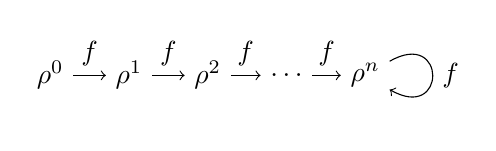
\begin{tikzpicture}
	\node (A) at (0,0) {$\rho^0$};
	\node (B) at (1,0) {$\rho^1$};
	\node (C) at (2,0) {$\rho^2$};
	\node (D) at (3,0) {$\ldots$};
	\node (E) at (4,0) {$\rho^n$};
	
	
	\draw[->] (A) -- node[above]{$f$} (B);
	\draw[->] (B) -- node[above]{$f$} (C);
	\draw[->] (C) -- node[above]{$f$} (D);
	\draw[->] (D) -- node[above]{$f$} (E);
	
	\draw[->] (E) edge [in=-30, out=30,looseness=6] node[right]{$f$} (E);
\end{tikzpicture}
\end{center}
\end{enumerate} 

\noindent Since we rely on the sequence to end in a fixpoint, so that we can end our abstract loop, we need to eliminate cases 1 and 2. For this we apply the widening operator $\triangledown$ after every loop pass. This operator is a function $\triangledown: \mathcal{R}_v\mapsto \mathcal{R}_v$, such that $f(\rho)\sqsubseteq\rho\triangledown f(\rho)$ and every infinite sequence $\rho^0,\rho^1,\dots$, where $\rho^n=\rho^{n-1}\triangledown f(\rho^{-1})$ is not strictly increasing \cite{cousot1977}. The exact definition of this widening operator depends on the used abstract domain.

\section{The Interval Domain}

\begin{figure}[!htb]
\begin{center}
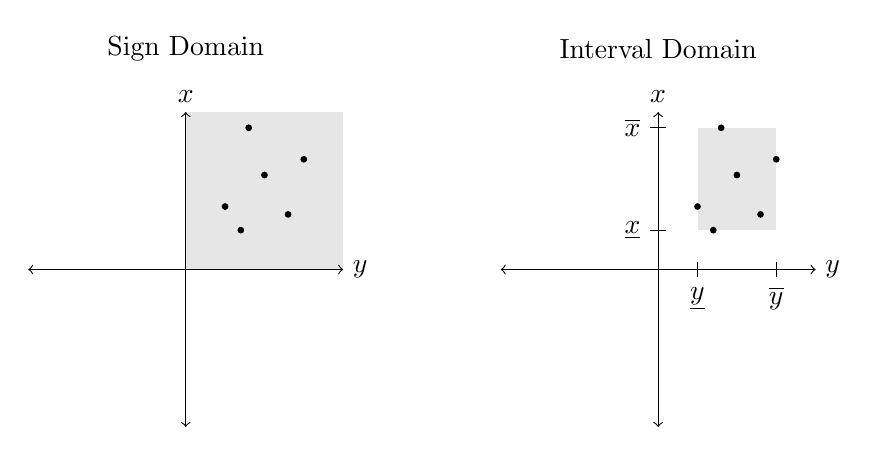
\begin{tikzpicture}
 		\coordinate (A) at (-1,-2);
		\coordinate (B) at (-1,2);
		\coordinate (C) at (-3,0);
		\coordinate (D) at (1,0);
		
		\draw [draw=none, fill=gray, fill opacity=0.2] (-1,0) -- (-1,2) -- (1,2) -- (1,0) -- cycle;
		
		%Axis
		\draw[<->] (A) -- (B) node [above] {$x$};
		\draw[<->] (C) -- (D) node [right] {$y$};
		
		
		\filldraw[black] (-0.5,0.8) circle (1pt);	
		\filldraw[black] (0,1.2) circle (1pt);
		\filldraw[black] (0.5,1.4) circle (1pt);	
		\filldraw[black] (-0.2,1.8) circle (1pt);
		\filldraw[black] (-0.3,0.5) circle (1pt);	
		\filldraw[black] (0.3,0.7) circle (1pt);	
		
		
		\node at (-1,2.8) {Sign Domain};
		
		\coordinate (E) at (5,-2);
		\coordinate (F) at (5,2);
		\coordinate (G) at (3,0);
		\coordinate (H) at (7,0);
		
		\draw [draw=none, fill=gray, fill opacity=0.2] (5.5,0.5) -- (5.5,1.8) -- (6.5,1.8) -- (6.5,0.5) -- cycle;
		
		\draw[-] (5.5,0.1) -- (5.5,-0.1);
		\draw[-] (6.5,0.1) -- (6.5,-0.1);
		
		\draw[-] (4.9,1.8) -- (5.1,1.8);
		\draw[-] (4.9,0.5) -- (5.1,0.5);
		
		\node at (5,1.8)[left, xshift=-1mm] {$\overline{x}$};
		\node at (5,0.5)[left, xshift=-1mm] {$\underline{x}$};
		
		\node at (5.5,0)[below, yshift=-1mm] {$\underline{y}$};
		\node at (6.5,0)[below, yshift=-1mm] {$\overline{y}$};
		
		%Axis
		\draw[<->] (E) -- (F) node [above] {$x$};
		\draw[<->] (G) -- (H) node [right] {$y$};
		
		\filldraw[black] (5.5,0.8) circle (1pt);	
		\filldraw[black] (6,1.2) circle (1pt);
		\filldraw[black] (6.5,1.4) circle (1pt);	
		\filldraw[black] (5.8,1.8) circle (1pt);
		\filldraw[black] (5.7,0.5) circle (1pt);	
		\filldraw[black] (6.3,0.7) circle (1pt);		
		
		\node at (5,2.8) {Interval Domain};		
		
		
\end{tikzpicture}
\end{center}
\caption{A diagram comparing abstract representation for a set of states. In this example a concrete state consists only of two scalar variable values $x$ and $y$. Therefore a concrete state can be represented as a point in the plane. The sign domain state, which is abstracting the marked concrete states, spans an entire quadrant of the coordinate system, whereas the interval domain state only occupies the rectangle encasing the states.}\label{fig:domaincomparison}
\end{figure}


\begin{figure}[htb]
	\begin{center}
		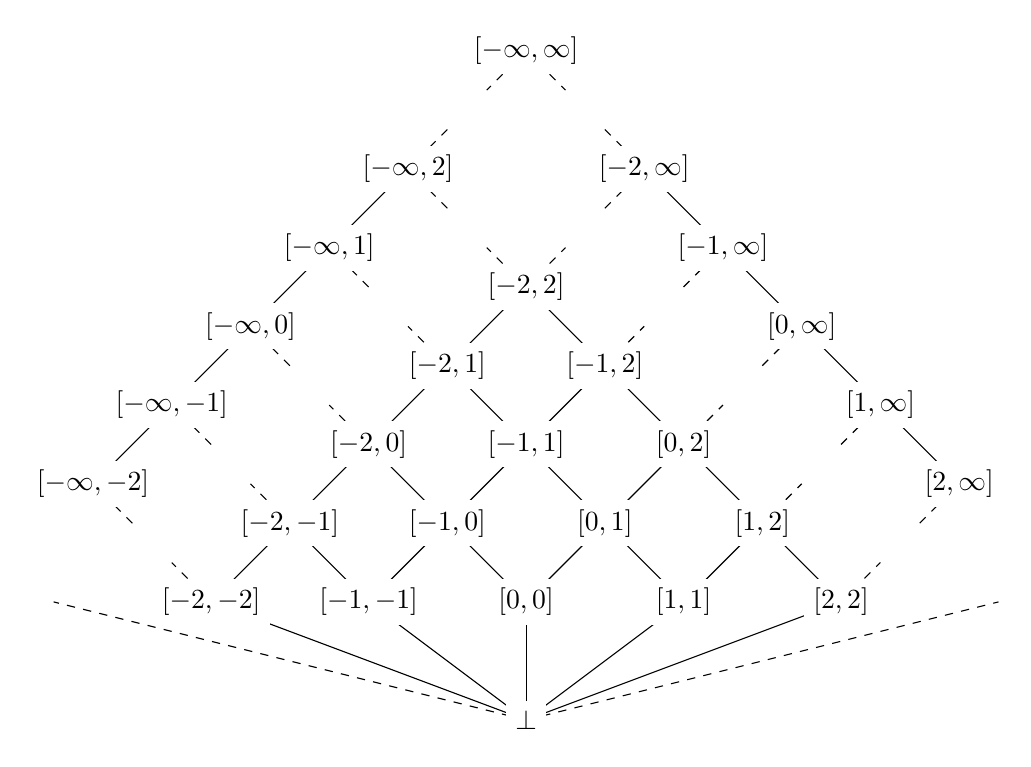
\begin{tikzpicture}
            \draw (0,0) -- (0,1.5);
            \draw (0,0) -- (2,1.5);
            \draw (0,0) -- (4,1.5);
            \draw (0,0) -- (-2,1.5);
            \draw (0,0) -- (-4,1.5);
            \draw (0,0)[dashed] -- (-6,1.5);
            \draw (0,0)[dashed] -- (6,1.5);
            
            \draw (2,1.5) -- (1,2.5);
            \draw (2,1.5) -- (3,2.5);
            \draw (4,1.5) -- (3,2.5);
            \draw (0,1.5) -- (1,2.5);
            \draw (0,1.5) -- (-1,2.5);
            \draw (-2,1.5) -- (-1,2.5);
            \draw (-2,1.5) -- (-3,2.5);
            \draw (-4,1.5) -- (-3,2.5);
            
            \draw (1,2.5) -- (0,3.5);
            \draw (1,2.5) -- (2,3.5);
            \draw (3,2.5) -- (2,3.5);
            \draw (-1,2.5) -- (0,3.5);
            \draw (-1,2.5) -- (-2,3.5);
            \draw (-3,2.5) -- (-2,3.5);
            
            \draw (2,3.5) -- (1,4.5);
            \draw (0,3.5) -- (1,4.5);
            \draw (0,3.5) -- (-1,4.5);
            \draw (-2,3.5) -- (-1,4.5);
            
            \draw (-1,4.5) -- (0,5.5);
            \draw (1,4.5) -- (0,5.5);
            
            \draw (-4,1.5)[dashed] -- (-4.5,2);
            \draw (-5,2.5)[dashed] -- (-5.5,3);
            
            \draw (-3,2.5)[dashed] -- (-3.5,3);
            \draw (-4,3.5)[dashed] -- (-4.5,4);
            
            \draw (-2,3.5)[dashed] -- (-2.5,4);
            \draw (-3,4.5)[dashed] -- (-3.5,5);
            
            \draw (-1,4.5)[dashed] -- (-1.5,5);
            \draw (-2,5.5)[dashed] -- (-2.5,6);
            
            \draw (0,5.5)[dashed] -- (-0.5,6);
            \draw (-1,6.5)[dashed] -- (-1.5,7);
           
            \draw (4,1.5)[dashed] -- (4.5,2);
            \draw (5,2.5)[dashed] -- (5.5,3);
            
            \draw (3,2.5)[dashed] -- (3.5,3);
            \draw (4,3.5)[dashed] -- (4.5,4);
            
            \draw (2,3.5)[dashed] -- (2.5,4);
            \draw (3,4.5)[dashed] -- (3.5,5);
            
            \draw (1,4.5)[dashed] -- (1.5,5);
            \draw (2,5.5)[dashed] -- (2.5,6);
            
            \draw (0,5.5)[dashed] -- (0.5,6);
            \draw (1,6.5)[dashed] -- (1.5,7);
            
            \draw (-5.5,3) -- (-1.5,7);
            \draw (5.5,3) -- (1.5,7);
            
            \draw (-1,7.5)[dashed] -- (-1.5,7);
            \draw (1,7.5)[dashed] -- (1.5,7);
            
            \draw (0,8.5)[dashed] -- (-0.5,8);
            \draw (0,8.5)[dashed] -- (0.5,8);
            
            \draw (0,0) node[fill=white!5] {$\perp$};
            \draw (0,1.5) node[fill=white!5] {$[0,0]$};
            \draw (2,1.5) node[fill=white!5] {$[1,1]$};
            \draw (4,1.5) node[fill=white!5] {$[2,2]$};
            \draw (-2,1.5) node[fill=white!5] {$[-1,-1]$};
            \draw (-4,1.5) node[fill=white!5] {$[-2,-2]$};
            
            \draw (1,2.5) node[fill=white!5] {$[0,1]$};
            \draw (3,2.5) node[fill=white!5] {$[1,2]$};
            \draw (-1,2.5) node[fill=white!5] {$[-1,0]$};
            \draw (-3,2.5) node[fill=white!5] {$[-2,-1]$};
            
            \draw (2,3.5) node[fill=white!5] {$[0,2]$};
            \draw (0,3.5) node[fill=white!5] {$[-1,1]$};
            \draw (-2,3.5) node[fill=white!5] {$[-2,0]$};
            
            \draw (1,4.5) node[fill=white!5] {$[-1,2]$};
            \draw (-1,4.5) node[fill=white!5] {$[-2,1]$};
            
            \draw (0,5.5) node[fill=white!5] {$[-2,2]$};
            
            
            \draw (-5.5,3) node[fill=white!5] {$[-\infty,-2]$};
            \draw (-4.5,4) node[fill=white!5] {$[-\infty,-1]$};
            \draw (-3.5,5) node[fill=white!5] {$[-\infty,0]$};
            \draw (-2.5,6) node[fill=white!5] {$[-\infty,1]$};
            \draw (-1.5,7) node[fill=white!5] {$[-\infty,2]$};
            
            
            \draw (5.5,3) node[fill=white!5] {$[2,\infty]$};
            \draw (4.5,4) node[fill=white!5] {$[1,\infty]$};
            \draw (3.5,5) node[fill=white!5] {$[0,\infty]$};
            \draw (2.5,6) node[fill=white!5] {$[-1,\infty]$};
            \draw (1.5,7) node[fill=white!5] {$[-2,\infty]$};
            
            \draw (0,8.5) node[fill=white!5] {$[-\infty,\infty]$};
         
        \end{tikzpicture}
        \caption{The interval abstract domain as a Hasse diagram \cite{cousot1977}}.\label{fig:intervaldomain}
	\end{center}
\end{figure}

Until this point we have been doing our abstract interpretation in the sign domain only. Let us introduce another, more precise one: The interval domain. This domain does not abstract the sign property of a scalar variable, but rather the property of which interval it is included in. An interval $[\underline{x},\overline{x}]$ has the concretisation $\gamma([\underline{x},\overline{x}])=\{z\in\mathbb{Z} \;|\; \underline{x}\leq z \leq \overline{x}\}$. Abstract expression operations follow usual interval arithmetics. For example, $[\underline{x},\overline{x}]+[\underline{y},\overline{y}]=[\underline{x}+\underline{y},\overline{x}+\overline{y}]$. Figure \ref{fig:domaincomparison} compares the sign domain to the interval domain and shows graphically how it abstracts in a more precise manner. Figure \ref{fig:intervaldomain} shows the interval lattice as a Hasse diagram.

\clearpage \section{The FunArray}

\subsection{Abstract Array Segmentation Predicates}

A FunArray predicate takes the form \funArray{\bound{e_1^1\ldots e_{m^1}^1} \fvalue{P_1} \bound{e_1^2\ldots e_{m^2}^2}[?^2] \fvalue{P_2}\ldots\allowbreak\fvalue{P_{n-1}}\allowbreak \bound{e_1^n\ldots e_{m^n}^n}[?^n]}, where $e^i_1\ldots e^i_m\in\mathbb{E}$ are expressions in normal form determining segment bounds, $P_i\in A$ are abstract element values from a chosen abstract domain $A$ and the optional $[?_i]$ signifies whether a preceding segment might be possibly empty \cite{cousot2011}. The FunArray maintains the condition that $e_1^1=\ldots=e_{m^1}^1\leq e_1^2=\ldots=e_{m^2}^2\leq\ldots\leq e_1^n=\ldots=e_{m^n}^n$, meaning that expressions in the same bound evaluate to an equal value and that the bounds are ordered. 
\vspace{0.2cm}
\begin{figure}[!htb]
\begin{center}
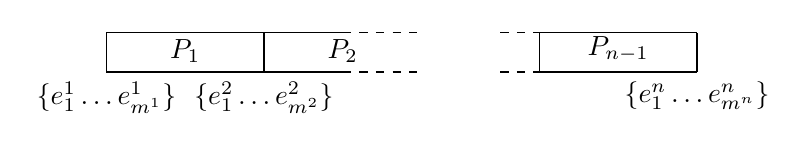
\begin{tikzpicture}

	\draw (0,0) -- (0,0.5);
	\draw (0,0) -- node[above]{$P_1$} (2,0);
	\draw (0,0.5) -- (2,0.5);
	\node[below] at (0,0) {$\{e_1^1\ldots e_{m^1}^1\}$};
	
	\draw (2,0) -- (2,0.5);
	\draw (2,0) -- node[above, xshift=0.5cm]{$P_2$} (3,0);
	\draw (2,0.5) -- (3,0.5);
	\node[below] at (2,0) {$\{e_1^2\ldots e_{m^2}^2\}$};
	\draw[dashed] (3,0) -- (4,0);
	\draw[dashed] (3,0.5) -- (4,0.5);
	
	
	\draw[dashed] (5,0) -- (5.5,0);
	\draw[dashed] (5,0.5) -- (5.5,0.5);
	\draw (5.5,0) -- (5.5,0.5);
	\draw (7.5,0) -- (7.5,0.5);
	\draw (5.5,0) -- node[above]{$P_{n-1}$} (7.5,0);
	\draw (5.5,0.5) -- (7.5,0.5);
	
	\node[below] at (7.5,0) {$\{e_1^n\ldots e_{m^n}^n\}$};
\end{tikzpicture}
\end{center}
\caption{Graphical representation of a the FunArray predicate.}\label{fig:funarraypredicate}
\end{figure}

\noindent Consider the following predicate for example: \funArray{A: \bound{0 \;\; a} \fvalue{[0,10]} \bound{a +4} \fvalue{[0,0]} \bound{b}?}. This means that the array $A$ has two segments. The first one which is bound by the expressions $0$ and $a$ on its left side and by $a+4$ on its right side. All array accesses with an index $i$ with $0=a\leq i \leq a+ 4$ will return the abstract value $[0,10]$. The second segment is bound by $a+4$ and $b$. It has the value $[0,0]$ and might possibly be empty as signified by the question mark.


\subsection{Functors}

An abstract domain functor is a function from the parameter domains $D_1,\ldots,D_n$ to a new abstract domain $D(D_1,\ldots,D_n)$ \cite{cousot2011}.
Since the FunArray is a functor $S(B(E),A,R)$, it can be adapted to a wide range of analyses by tweaking its parameter domains. It takes the following domains as arguments:
\begin{itemize}[label={--}]
	\item The segment bound $B(E)$, which in turn is also a functor from the expression domain $E$.
	\item The array element abstract domain $A$. This is an arbitrary abstraction on the examined values. In the remaining examples in this thesis, this is going to be the interval domain.
	\item The variable abstract domain $R$.
\end{itemize} 

\subsection{Abstract operations}

As an abstract domain, the FunArray supports the abstract operations join $\sqcup$, meet $\sqcap$, partial order $\sqsubseteq$, widen $\triangledown$ and narrow $\vartriangle$. To apply these, the segment bounds of the triangle need to be unified and the respective operation applied segment wise. Unification is a process whereby the FunArrays $A$ and $B$ are modified into $A'$ and $B'$, such that $A\sqsubseteq A'$ and $B\sqsubseteq B'$ and the segment bounds for $A'$ and $B'$ are identical.


\subsection{Transformers}

An array access \texttt{A[e]} in the FunArray domain is not as trivial as in a concrete execution of a program. Because \texttt{e} might not actually be present in the bounds of the FunArray, we need to find the greatest bound $B_l\leq \llbracket \texttt{e}\rrbracket$ and the least bound $B_g\geq \llbracket \texttt{e}\rrbracket$ in a given array. The evaluation of the array access is then $\llbracket\texttt{A[e]}\rrbracket=\bigsqcup^{g-1}_{k=l}P_k$.

An array is modified by the array assignment \texttt{A[i] = e}. Its semantics is defined as follows: $\llbracket\texttt{A[i] = e}\rrbracket\rho=\rho[A:=A']$, meaning the array $A: B_1P_1B_2[?_1]\ldots P_{n-1}\allowbreak{}B_n[?_{n-1}]$ has been replaced by the modified $A': B_1P_1B_2[?_1]\ldots\allowbreak B_l[?_l] (\bigsqcup^{g-1}_{k=l}P_k)\allowbreak\, \{\,\llbracket\texttt{i}\rrbracket\,\}?\, \llbracket\texttt{e}\rrbracket \allowbreak\,\{\,\llbracket\texttt{i}\rrbracket+1\,\}\, \allowbreak(\bigsqcup^{g-1}_{k=l}P_k) B_g?\ldots \allowbreak P_{n-1}B_n[?_{n-1}]$, whereby $B_l\leq\llbracket\texttt{i}\rrbracket\leq B_g$.

When modifying variables in the state, the FunArray predicates also need to be modified as they might contain that variable. consider an array \funArray{A: \bound{a} \fvalue{P_1} \bound{b} \fvalue{P_2} \bound{c}}. If there is an assignment \texttt{b := b+1}, the FunArray needs to be modified to \funArray{A': \bound{a} \fvalue{P_1} \bound{b-1} \fvalue{P_2} \bound{c}}, so that it is still correct. 
















\chapter{Implementation}
\section{Scalar Variables}\label{sec:scalarvariables}
Cousot, Cousot and Logozzo's FunArray is embedded into Clousot, an already existing static code contract analyser for the .NET framework \cite{cousot2011}. It therefore profits from an already existing abstract analysis for scalar variables. My implementation however works in a rudimentary standalone analyser and implements its own abstract domains for scalar variables.
They are defined by the interface \texttt{DomainValue} and support only a limited amount of arithmatic operations: Addition, subtraction, multiplication, division, modulo, negation and absolute value. Operations like exponentiation or bitwise xor etc. that are available in many programming languages like C or Java, have not been implemented, which limits the amount of programs that can be analysed with my implementation. 

Since the focus of my work is to test the FunArray technique I have refrained from implementing more complicated abstract domains (that would have delivered more precise results), like for example the relational approach of polyhedra \cite{cousot1978}. Instead I primarily focused on the interval domain. To prove that the FunArray works with different scalar variable abstractions I also partially implemented the sign domain.

\subsection{Intervals}
I chose to only abstract integers with this domain, as the use of floating point numbers and open intervals would introduce unnecessary inaccuracies and the benchmark I later tested against only included integers as well. The implementation of the interval domain is relatively straight-forward. An interval $[a,b]$ consists of a lower limit $a$ and an upper limit $b$ with $a,b \in \mathbb{Z}\cup\{-\infty,\infty\}$. The set of $\mathbb{Z}\cup\{-\infty,\infty\}$ is implemented by the \texttt{InfInt} class. It allows calculations on infinities, such as $\infty - 10 = \infty$ or $(-4) \cdot \infty = -\infty$, by extending the operations of arithmetics in $\mathbb{Z}$. It is assumed that there are no integer overflows.

\subsubsection{Arithmetic Expression Operations}
Table \ref{table:intervalarithmetics} shows the supported expression arithmetics for the \texttt{ReachableInterval} class and how they are implemented. Most operations are intuitive and follow the classical interval arithmetic \cite{dawood2011}. Operations with at least one of the operands being of the class \texttt{Unreachable} representing $\bot$, yield another \texttt{Unreachable}. 

The abstraction of the modulo operation is not as straight-forward as the others. Different programming languages define their modulo operator differently. For example \texttt{7 \% -5} in C or Java yields a result of $2$ whereas the same expression in Python yields $-3$. Both results are mathematically correct, because $2 \equiv -3 \mod -5$, when talking about equivalence classes. The programming languages just translate those equivalence classes differently into integers. I chose for my interval domain to follow the semantics of C, where the sign of the result of a modulus operation is equal to the dividend's sign. The modulo operation also over-approximates the result for ease of implementation.

\begingroup
\renewcommand{\arraystretch}{1.3}
\begin{table}[hbt]
\begin{center}
\begin{tabular}{l|l}
           negation & $-[\underline{x},\overline{x}]=[-\overline{x},-\underline{x}]$\\
           \hline
           scalar addition & $s + [\underline{x},\overline{x}] = [s+ \underline{x}, s+ \overline{x}]$\\
           \hline
           addition & $[\underline{x},\overline{x}]+[\underline{y},\overline{y}]=[\underline{x} + \underline{y},\overline{x}+\overline{y}]$\\
           \hline
           scalar subtraction & $s - [\underline{x},\overline{x}] = [s- \overline{x}, s- \underline{x}]$\\
           & $[\underline{x},\overline{x}]-s = [\underline{x}-s, \overline{x}-s]$\\
           \hline
           subtraction & $[\underline{x},\overline{x}]-[\underline{y},\overline{y}]=[\underline{x} - \overline{y},\overline{x}-\underline{y}]$\\
           \hline
           scalar multiplication & $s\cdot[\underline{x},\overline{x}]=[\min(s\cdot\underline{x},s\cdot\overline{x}), \max(s\cdot\underline{x},s\cdot\overline{x})]$\\
           \hline
           multiplication & $[\underline{x},\overline{x}]\cdot[\underline{y},\overline{y}]=$\\
           &$\qquad[\min(\underline{x}\underline{y}, \underline{x}\overline{y}, \overline{x}\underline{y}, \overline{x}\overline{y}), \max(\underline{x}\underline{y}, \underline{x}\overline{y}, \overline{x}\underline{y}, \overline{x}\overline{y})]$\\
           \hline
           scalar Euclidean division & $s \div [\underline{x},\overline{x}] = [\min(s \div \overline{x}, s \div \underline{x}), \max(s \div \overline{x}, s \div \underline{x})]$\\
           & $[\underline{x},\overline{x}]\div s = [\min(\underline{x}\div s, \overline{x}\div s),\max(\underline{x}\div s, \overline{x}\div s)]$\\
           \hline
           Euclidean division & $[\underline{x},\overline{x}]\div[\underline{y},\overline{y}]=[\min(\underline{x}\div\underline{y}, \underline{x}\div\overline{y}, \overline{x}\div\underline{y}, \overline{x}\div\overline{y}),$\\
           &$\qquad\max(\underline{x}\div\underline{y}, \underline{x}\div\overline{y}, \overline{x}\div\underline{y}, \overline{x}\div\overline{y})]$\\
           \hline
           scalar modulo & $[\underline{x},\overline{x}]\;\%\; s = [\underline{x} \;\%\; s,\overline{x} \;\%\; s]$\\
           \hline
           modulo & $[\underline{x},\overline{x}]\;\%\;[\underline{y},\overline{y}]$ \\
           & $\qquad=\begin{cases}
           [0, \min(\overline{x},\overline{x})],& \text{if } \underline{x}\geq 0\\
           [\max(\underline{x},-\underline{y}),0],& \text{if } \underline{x}< 0 \wedge \overline{x} < 0\\
           [\min(\overline{x},\overline{x}), \max(\underline{x},-\underline{y})],& \text{otherwise}
           \end{cases}$\\
           \hline
           absolute value & $ \mathrm{abs}([\underline{x},\overline{x}]) $\\
           &$\qquad=
           \begin{cases}
           [0,\max(-\underline{x}, \overline{x})],& \text{if } \underline{x}< 0 \wedge \overline{x}\geq 0\\
           [0,\max(-\underline{x}, -\overline{x})],& \text{if } \underline{x}< 0 \wedge \overline{x}< 0\\
           [\underline{x},\overline{x}]	,& \text{otherwise}
           \end{cases}
           $
           
           
        \end{tabular}
  \caption{Supported expression operations for the implemented interval domain. This is a simplified overview and leaves out a lot of edge cases (e.g. division by zero, infinities etc.). It is assumed that the intervals are non-empty/reachable.}\label{table:intervalarithmetics}
  \end{center}
\end{table}
\endgroup

\subsubsection{Abstract operations}
Table \ref{table:intervalabstractoperations} shows the implementations of the abstract operations for the \texttt{Interval} class. The join $\sqcup$ and meet $\sqcap$ are basically equivalent to their concrete set operations $\cup$ and $\cap$. When the result of a meet operation $[\underline{x},\overline{x}] \sqcap [\underline{y},\overline{y}] = [\underline{z},\overline{z}]$ would be an illegal interval, such that 
$\underline{z}>\overline{z}$, instead an \texttt{Unreachable} is returned.

\begingroup
\renewcommand{\arraystretch}{1.3}
\begin{table}[htb]
\begin{center}
\begin{tabular}{l|l}
		   operation & implementation\\
		   \hline
           join & $[\underline{x},\overline{x}]\sqcup[\underline{y},\overline{y}]=[\min(\underline{x},\underline{y}),\max(\overline{x}, \overline{y})]$\\
           \hline
           meet & $[\underline{x},\overline{x}]\sqcap[\underline{y},\overline{y}]=[\max(\underline{x},\underline{y}),\min(\overline{x}, \overline{y})]$ \\&\qquad or $\bot$, if $\max(\underline{x},\underline{y})>\min(\overline{x}, \overline{y})$\\
           \hline
           widening& $[\underline{x},\overline{x}]\triangledown[\underline{y},\overline{y}]=\left[\left(
           \begin{cases}
           	-\infty,& \text{if } \underline{y} < \underline{x}\\
           	\underline{x},& \text{otherwise}
           \end{cases}
           \right),\left(
           \begin{cases}
           	\infty,& \text{if } \overline{y} > \overline{x}\\
           	\overline{x},& \text{otherwise}
           \end{cases}
           \right)\right]$
           
           
        \end{tabular}
  \caption{Supported abstract operations for the  implemented interval domain \cite{cousot1976}.} \label{table:intervalabstractoperations}
  \end{center}
\end{table}
\endgroup

\subsubsection{Abstraction and Concretisation Functions}
The abstraction function defined in the \texttt{Domain} deviates from the mathematical definition as explained in section \ref{sec:abstractinterpretation:abstraction}. Instead of abstracting from a property (a set of integers), it abstracts from a single integer, since a concrete program only deals with integers but not with sets. The abstraction function is needed when evaluating an expression containing constants as described in section \ref{sec:expressions:evaluation}. It is implemented as $\alpha(z)=[z,z]$.
The concretisation function $\gamma$ deviates in the same way and can only concretise intervals $\gamma([\underline{z},\overline{z}])=z$ where $z = \underline{z} = \overline{z}$. When $\underline{z} \neq \overline{z}$, the method throws a \texttt{ConcretisationException}. The concretisation function is needed for normalising expressions as described in section \ref{sec:expressions:normalisation} and the exception is being handled in that process. 

\subsection{Signs}
I also partially implemented the Sign domain to make sure that my implementation of the FunArray works as intended with different abstractions of element values. The \texttt{Sign} class however does not implement all methods defined in the \texttt{DomainValue} interface and cannot be used in a full analysis of a program.





\section{Arrays}

The \texttt{FunArray} class provides a collection of bounds, element values and segment emptiness information. I decided against implementing the FunArray as a linked list and instead stored these values in Java collections as to make use of the Java stream API. The emptiness information is stored as boolean values (a segment can either be might-be-empty or non-empty). Array elements can take any implementation of the \texttt{DomainValue} (See section \ref{sec:scalarvariables}). Bounds are stored as \texttt{Bound} objects. The \texttt{FunArray} is immutable and when changed provides modified copies of itself.

Apart from some minor utility methods, the \texttt{FunArray} provides four major methods: \texttt{get}, \texttt{insert}, \texttt{join} and \texttt{widen}. The \texttt{get} method takes a normal expression as an argument and returns the element value at that index. Since that very index might not necessarily be present in the bounds, this operation is not as trivial as it sounds. The array is traversed from the left and the rightmost bound that can be said to be less than the given index is being searched. After that, the array is traversed from the right and the leftmost bound that is greater than the index plus one is found. The result of the \texttt{get} operation then is the join of all array elements that lie between both these bounds. If it is not possible to find bounds less or greater than the given index, instead the most outer bounds of the array are being used, as it is simply assumed that no array access is ever out of bounds. The \texttt{insert} method works in a similar way. Since the desired index might not actually be present in the bounds of the array, it is not possible to directly insert the designated value. Instead, once again, the rightmost bound smaller than the index and the leftmost bound greater than the index are being searched. The bounds between them are being removed and the values between them are joined. Then a new segment with the desired value is placed in the middle of this joined segment \cite{cousot2011} . Consider an Array $A$, looking like $B_1P_1B_2[?_1]\ldots P_{n-1}B_n[?_{n-1}]$, where $B_n$ is the $n$-th bound, $P_n$ is the $n$-th value and $[?_{n}]$ is the emptiness flag for the $n$-th segment. We want to insert a value $v$ at the index $i$. The rightmost bound smaller than the index $B_l$ and the leftmost bound greater than the index $B_g$ are determined and the segments in between are being joined: $B_1P_1B_2[?_1]\ldots B_l[?_l] (\bigsqcup^{g-1}_{k=l}P_k) B_g[?_g]\ldots P_{n-1}B_n[?_{n-1}]$. Then the desired value  is inserted in this joined segment like this: $B_1P_1B_2[?_1]\ldots\allowbreak B_l[?_l] (\bigsqcup^{g-1}_{k=l}P_k)\allowbreak\, \{\,i\,\}?\, v \,\{\,i+1\,\}\, \allowbreak(\bigsqcup^{g-1}_{k=l}P_k) B_g?\ldots \allowbreak P_{n-1}B_n[?_{n-1}]$. Edge cases in which for example $i\in B_l$ are being handled, but won't be described any further here. The \texttt{join} and \texttt{widen} operations first execute a unification as described in section \ref{sec:funarray:unifying} and then join or widen the element values segment wise.

\textcolor{red}{Evtl diesen Part eher in den Background packen. Ist zwar so auch implementiert, aber ist eigentlich nicht von mir ausgedacht worden. Hier in dieser Section nur drauf eingehen, wies denn eigentlich implementiert wurde. Bzw evtl diesen Part weiter nach hinten verschieben in die Assignment Section}

\subsection{Bounds and Normal Expressions}

Expressions that appear in the bounds of a FunArray follow a chosen normal form. These are implemented separately from the arithmetic program expressions described in section \ref{sec:expressions} in the class \texttt{NormalExpression}. This split design was chosen because the bound expression need to fulfil some additional functionality like syntactic comparison. I adapted Cousot, Cousot and Logozzo's normal form of $\mathtt{v}+k$, where \texttt{v} is a \texttt{Reference} and $k$ is a constant integer value \cite{cousot2011}. The \texttt{Reference} interface is implemented by the \texttt{VariableReference} class, which is nothing more than a wrapper for a string, representing a variable name, and the \texttt{ZeroReference}, which is a special variable whose value is assumed to always be zero, such that it is possible to represent constants as normal expressions. Two normal expressions can be syntactically compared if their variable reference is the same, by simply comparing their constant value. A refinement that has not been made in my implementation would be to semantically compare bound expressions. This syntactical comparison is needed when getting or inserting a value into a FunArray.

The \texttt{Bound} class is a wrapper for a set of \texttt{NormalExpression} that provides some set algebra (union, intersection etc.) as this is not part of the standard Java set. It also provides functionality to modify the bound accordingly when a variable value changes (a new expression needs to be added, when a variable value is set to a value already present in that bound for example).

\subsection{Unifying two FunArrays}\label{sec:funarray:unifying}

Cousot, Cousot and Logozzo developed a recursive algorithm for unifying two FunArray segmentations \cite{cousot2011}. It is subjectively complicated to understand at first glance and needs to handle 11 different distinct sub-cases. It is a recursive algorithm that relies on the assumption that the left side of the array is already unified, but in one case that assumption is violated, making it hard to actually implement it recursively. When I implemented it, it was also prone to errors and hard to debug. Therefore I chose to implement the unifying of two segmentations in a different iterative algorithm. The authors also mentioned that they refined their algorithm in their actual implementation of the FunArray, mentioning a ``purification step'' that sounds similar to my approach, but don't go into more detail \cite[section 12.2]{cousot2011}. As their implementation is not freely available, one could only guess that they might have actually taken a similar approach as me in the end. My algorithm works as follows:
\begin{enumerate}
  \item Consider two FunArrays $A=B_{A1}P_{A1}B_{A2}[?_{A1}]\ldots B_{An}[?_{An-1}]$ and $B=B_{B1}\allowbreak P_{B1}\allowbreak B_{B2}\allowbreak[?_{B1}]\ldots B_{Bm}[?_{Bm-1}]$, with bounds $B$ being treated as sets of expressions $\{\mathtt{e}_1, \mathtt{e}_2,\ldots\}$. Also consider their respective neutral elements $\nElement_A,\nElement_B\in \{\bot,\top\}$
  \item Replace all $B_{Ai}$ with $B_{Ai}\cap(B_{B1}\cup B_{B2}\cup\ldots)$, therefore removing all expressions in the bounds of $A$ and $B$ that are only present in either of them but not both.
  \item \label{item:removeemptybounds} If that leaves empty bounds, such that $B_{i}=\emptyset$, remove that bound and merge the adjacent segment values via the join operation. The Array
  $X = \ldots B_{i-1}[?_{i-2}]\allowbreak P_{i-1} \allowbreak B_{i} [?_{i-1}] P_{i} B_{i+1} [?_{i}]\ldots$
  then becomes 
  $X'=\ldots B_{i-1}[?_{i-2}] \allowbreak P_{i-1}  \,\sqcup\, P_{i} B_{i+1} [?_{i-1} \,\sqcup\, ?_{i}]\ldots$
  \item Now traverse the bounds of both FunArrays from left to right.
  \begin{enumerate}[label*=\arabic*.]
    \item If $B_{Ai} \cup B_{Bi} = \emptyset$, replace $B_{Ai}$ and $B_{Bi}$ with empty bounds and go on to the next bounds $B_{Ai+1}$ and $B_{Bi+1}$.
    \item If $B_{Ai} \cup B_{Bi} \neq \emptyset$, add a neutral segment, so that $A=\ldots B_{Ai}P_{Ai}\allowbreak B_{Ai+1}\ldots$ becomes $A'=\ldots (B_{Ai} \cup B_{Bi}) \;\nElement_A\, (B_{Ai} \setminus B_{Bi}) P_{Ai}B_{Ai+1}\ldots$. Skip this if $B_{Ai} \setminus B_{Bi}=\emptyset$. Add a segment with value $\nElement_B$ in $B$ analogously.
  \end{enumerate}
  \item Finally remove all empty bounds in the resulting FunArrays, as described in Step~\ref{item:removeemptybounds}.
\end{enumerate}

\noindent The two resulting FunArrays $A'$ and $B'$ have an identical segmentation, meaning their bounds are the same in the same order. The algorithm only ever introduces new segments with a value $\nElement\in\{\bot,\top\}$, that might be empty. When the value of that element is $\top$, the resulting Array $A'$ is an over-approximation of $A$. When that element is $\bot$, the resulting Array $A'$ is actually equal to $A$, as their are no concrete values, that are abstracted by $\bot$ and the segment therefore must be empty. We can therefore say that the resulting Arrays from this algorithm are over-approximations of their respective predecessors: $A\sqsubseteq A'$ and $B\sqsubseteq B'$.

\subsubsection{Example unification}






\section{States}





\section{Arithmetic Expressions}\label{sec:expressions}

Arithmetic expressions are defined in the \texttt{Expression} interface. I implemented the three atomic expressions \texttt{Constant}, \texttt{Variable} and \texttt{ArrayElement} and the five expression operations \texttt{Addition}, \texttt{Subtraction}, \texttt{Multiplication}, \texttt{Division} and \texttt{Modulo}. 

\subsection{Evaluation of an Expression}\label{sec:expressions:evaluation}
Evaluating an expression is basically the same as determining its abstract semantics under the current state. Since the \texttt{DomainValue} class has the five arithmetic operations already defined as methods, the evaluation implementation of the expression operations is obvious. The evaluation of the three atomic expressions however is not as simple. Since the FunArray allows differing value domains for variables and its elements, it might not possible to calculate with those straight-away. The constant expression represents a concrete constant value and therefore lies in yet another domain. Cousot, Cousot and Logozzo chose to evaluate their expressions in the variable domain \cite{cousot2011}. There is no immediately obvious reason as to why an evaluation in the array element domain should not be considered, but I chose to follow their lead nevertheless. Therefore, two translation functions are needed to translate the concrete constant values and the array element values into the appropriate value in the variable value domain. The former is simply the abstraction function $\alpha$ which is provided by the \texttt{Domain} class and the latter called \texttt{convert\allowbreak{}Array\allowbreak{}Element\allowbreak{}Value\allowbreak{}To\allowbreak{}Variable\allowbreak{}Value} is provided by the \texttt{AnalysisContext}interface. When both variables and array elements are being abstracted into the same domain, this is simply the identity function. Its opposite, \texttt{convert\allowbreak{}Variable\allowbreak{}Value\allowbreak{}ToArray\allowbreak{}Element\allowbreak{}Value}, is needed when the calculated value of an expression is supposed to be assigned to an array element.


\subsection{Normalisation of an Expression}\label{sec:expressions:normalisation}

Since general expressions (that are not already in normal form) are being used as indeces when assigning a value to an array element, they need to be able to be brought into normal form. This works differently for different expressions. Some expressions may be able to be brought into more than one normal form or none at all. Consider the expression \texttt{e = a + b} and the state $\rho=\{\mathtt{a}\mapsto[3,3], \mathtt{b}\mapsto[7,7]\}$ for example. There are actually 3 ways \texttt{e} can be written in our $\mathtt{v}+k$ normal form: $\mathtt{a}+7$, $\mathtt{b}+3$ or $\mathtt{v_0}+10$, where $\mathtt{v_0}$ is a special variable whose value is always assumed to be zero. All three of these are being considered when inserting a value into an array.

\subsubsection{Addition and Subtraction}


Consider an addition expression $\mathtt{a}=\mathtt{e}_1 + \mathtt{e}_2+\ldots+\mathtt{e}_n$. Its normal forms are derived the following way:


\begin{enumerate}
	\item Consider a single normal form $\mathtt{v}_i + k_i$ of a single summand $\mathtt{e}_i$.
	\item Evaluate the expression $\mathtt{a}'=\mathtt{e}_1 +\ldots+ \mathtt{e}_{i-1} + \mathtt{e}_{i+1} +\ldots+\mathtt{e}_n+k_i$.
	\item If its value is concretisable, meaning it can be concretised into a single integer value (e.g. $\gamma([3,3])=3$), add $\mathtt{v}_i+\gamma(\llbracket\mathtt{a}'\rrbracket)$ to the list of normal forms for \texttt{a}.
	\item Repeat for all operands \texttt{e} in \texttt{a}. 
\end{enumerate}

\noindent The normalisation of subtraction works the same way, since a subtraction is nothing more than an addition with exactly two operands where the value of the second operand is being inverted when evaluating.

\subsubsection{Variable and Constant}
Normalising a constant expression \texttt{k} is trivial, as its normal form is simply $\mathtt{v_0}+k$, where $\mathtt{v_0}$ is a special variable whose value is assumed to always be zero of the class \texttt{ZeroReference}. Equally as trivial is the normalisation of a variable expression \texttt{v}. Its normalisation is $\mathtt{v}+0$. If $\llbracket\mathtt{v}\rrbracket$ is concretisable, meaning it describes a single concrete value $k'$, the second normal form of \texttt{v} is $\mathtt{v_0}+k'$.


\subsubsection{Multiplication, Division, Modulo and Array Element}

The normalisation of the multiplication, division and modulo expressions is quite similar to the constant normalisation. As there es no general way to rearrange them into normal form, they can only be normalised, when their evaluation can be concretised into the constant part of the normal form. Of course there are certain refinements that could be done here, like rearranging multiplications into additions when a factor can be concretised. These opportunities have not been seized to keep the process of normalisation as simple as possible and as these refinements would probably only yield a marginal reward. 






\section{Assignments}






\section{Conditionals}\label{sec:conditions}

When defining the semantics of a real world programming language like C, we would normally not only need to assign semantics to arithmetic expressions like in the previous section, but also to boolean expressions \cite{scott1971}. As my analyser is not going to be used to analyse C programs or programs in any other real world programming language directly, I skipped this step. This means my analyser is only able to work with conditionals that are simple comparisons of arithmetic expressions. It is however possible to emulate boolean expressions by clever use of control structure. For example a conjunction is equivalent to a nested if-then-else statement and a negation is equivalent to the complement relation condition.

When executing a program containing a conditional in the concrete, it is possible to determine whether the condition is satisfied or not and so, only one program branch has to be executed at a time. When interpreting it in the abstract, it is often not possible to determine this. Consider the condition \texttt{x~>=~0} for example. Under the abstract state $\rho=\{\mathtt{v}\mapsto[-1,1]\}$, this question is undecidable, as for some concrete values it true and for other it is false. The solution therefore is to execute both branches, assume the condition to be true and false respectively and in the end join the states of both branches.

\noindent\textcolor{red}{TODO}





\section{Loops}

\chapter{Evaluation}\label{chap:evaluation}

To evaluate my implementation of the FunArray, we will experimentally test it. We want to determine its effectiveness in determining loop invariants, as well as in asserting given proof obligations.

\section{Experimental Setup}
\subsection{Benchmarks}

The International Competition on Software Verification (or SV-COMP)\footnote{More information about SV-COMP available at \url{https://sv-comp.sosy-lab.org/}} provides a set of benchmarks that can be used to compare tools for software verification\footnote{Available at \url{https://gitlab.com/sosy-lab/benchmarking/sv-benchmarks}}. Their subcategory ``c/ReachSafety-Arrays'' contains a collection of 433 verification tasks written in C for which the treatment of arrays is necessary to determine reachability. As such, this collection is suitable to test my implementation of the FunArray. They include at least one assertion per benchmark and its expected verdict for testing.
The simple C programs have been translated to the embedded domain-specific language in Java using the tool Cuv\'ee \cite{ernst2020}. Since my implementation of the FunArray does not provide the entire functionality of the C language, about half of the benchmarks could not be translated. The 196 untranslatable benchmarks utilise features like the use of boolean variables, nested arrays, functions with a return value, structs and the use of the break keyword.

\subsection{Formal Arguments of the FunArray}

One of the FunArray's strengths is its ability to use different abstract domains for its bounds, array elements and variables without having to adapt the static analyser. For this evaluation the following abstract domains have been chosen as the FunArray functor's formal arguments: For abstracting variables and array elements the interval domain has been chosen, since it is relatively simple to implement. The chosen expression domain and therefore the abstract representation of segment bounds follows the scheme used by the FunArray's inventors \cite[section 7.2]{cousot2011}. Expressions are limited to the normal form $v+k$ where $v$ is a variable (whose value is abstracted by intervals) and $k$ is an integer constant.

\section{Results}

The execution time of the benchmarks is almost negligible. To execute all 237 benchmarks it takes 253 milliseconds (Averaged value over 100 runs. The workbench used is a M2 Max MacBook Pro running OpenJDK 22). This comes down to about a millisecond per benchmark. This result was expected, since the FunArray does not handle disjunctions separately but through the use of empty segments. No combinatorial explosion is expected to occur.

\subsection{Definition of Triviality}

We want to determine for how many of the benchmarks' loops the analyser is able to come up with an invariant. Since the analysis will always produce a result even if there is no meaningful information that can be extracted from it, we need to define triviality for these results. Consider an array $A$ for example. The analysis is run on some some loop and determines the invariant for $A$ to be \funArray{A:\bound{a} \fvalue{[-\infty,\infty]} \bound{a.length}?}. This basically tells us that $A$ contains integers whose value is entirely unknown on its entire length, or in other words: We know nothing at all about \texttt{A}. Therefore this invariant must be considered trivial. More generally, a state containing only arrays that themselves only contain segments of unknown value is certainly considered trivial.

What we consider non-trivial is however not as clear. It might seem intuitive to consider every state that does not fit this description as such, however this leaves out an important aspect: The FunArray analyser is able to fully automatically divide an array into semantic segments. This differentiates the FunArray from a technique called array smashing \cite{cousot2011}. An analysis employing array smashing treats all array elements homogeneously. When changing a single element value, its abstract value is joined with all other elements and a lot of information is lost that way. To evaluate in which cases the FunArray analyser beats the array smashing, we must consider two different types of non-triviality:

\begin{enumerate}
	\item The general case, where at least one array in a state contains at least one segment with a value more specific than $\top$.
	\item The more narrow case where at least one array is two or more segments long and at least one of these segments has a value more specific than $\top$.
\end{enumerate}

\noindent Of course it is not assured that we could have determined the same invariant via array smashing in the first case, but we certainly know that we could not have gotten the same result in the second case without the automatic semantic segmentation.


\subsection{Invariants}

Spread across the 238 benchmarks there are 947 loops. For 580 or 61.3\% of those my implementation of the FunArray was able to determine a general non-trivial invariant. When examining the more narrow requirements for non-triviality, we arrive at 427 invariants, which is still 45.0\% of the total, meaning the FunArray is able to generate at least four times as many non-trivial invariants as the array smashing technique. If we were to increase the required number of segments to more than two, this number would drop down to 3, suggesting the FunArrays ability to depict a lot of segments cannot be utilised in actual code analyses. No calculated invariants had more than three segments.

\subsection{Verifying assertions}

My implementation is able to correctly identify the result of 24 out of the 247 assertions spread among 237 benchmarks or 9.7\% of assertions. It did not contradict any proof obligations. When manually inspecting the program mechanism preceding these assertions in the benchmark, a single pattern can be identified that precedes the majority of them: Initialisation. The benchmark first initialises an array with a consistent value as its every element and immediately afterwards asserts that every element of the array has that specific value. Of the 24 correctly assessed assertions, 20 follow this pattern. The remaining four assertions follow a more complex program scheme, that involves conditions and loops. This suggests that one of the strengths of the FunArray is to recognise correct initialisation of arrays.



\section{Discussion}
\subsection{Comparison with Cousot, Cousot and Logozzo's Results}

Cousot, Cousot and Logozzo evaluate their implementation of the FunArray by analysing the main libraries of the .NET framework and the implementation itself \cite{cousot2011}. The .NET libraries have been chosen for this since they contain a large amount of code and a vast selection of functionalities and techniques. They, however, lack an important aspect: The specification of expected properties. The authors are able to infer thousands of invariants but cannot determine whether they actually provide any useful information for the further execution of the code. To check against pre-specified properties they annotated their implementation of the FunArray with pre-conditions and proof obligations and ran it on itself. They were able to correctly assert 61 out of 1800 or 3.4\% of proof obligations when analysing the FunArray implementation using itself \cite{cousot2011}. This roughly matches my results of 9.7\%, considering the easy initialisation assertions make up a way greater amount of my test cases than would be present in a real world program.

\subsection{Limitations}

\subsubsection{Adjacent potentially empty segments}
When expanding a segment by inserting a value adjacent to it, formerly adjacent and potentially empty segments will be joined with their nearest neighbour until a non-empty segment is reached. Let us consider the FunArray \funArray{A:\bound{a} \fvalue{x} \bound{b} \fvalue{y} \bound{c}? \fvalue{z} \bound{d}} for example. It is unknown whether its second segment containing the value $y$ is empty or not and thus whether $b=c$ or $b<c$ is true.
When trying to expand the first segment by inserting its value $x$ at index $b$, the resulting FunArray could either be \funArray{\bound{a} \fvalue{x} \bound{b\;c} \fvalue{x} \bound{b+1}? \fvalue{z} \bound{d}}, if the $y$-segment was empty, or alternatively \funArray{\bound{a} \fvalue{x} \bound{b} \fvalue{x} \bound{b+1} \fvalue{y} \bound{c}? \fvalue{z} \bound{d}}, if it was non-empty. Since the position of the \funArray{\bound{c}}-bound cannot by decided, it must be discarded altogether. After the insertion, $A$ becomes \funArray{A':\bound{a} \fvalue{x} \bound{b} \fvalue{x} \bound{b+1}? \fvalue{y\sqcup z} \bound{d}} and all information concerning the variable $c$ is lost.
Analyses of programs utilising segments in their arrays with adjacent and potentially empty segments have to discard non-trivial information. Thus the FunArray's approach for handling potentially empty adjacent segments limits the number of programs for which an analysis can achieve a non-trivial result. Consider the following program, a C implementation of Dijkstra's Dutch national flag algorithm \cite{dijkstra1976}, for example. This example is not one of the benchmarks, but rather an algorithm that I tried to run while debugging and which turned out to not be analysable by my implementation in a meaningful way.
 
\vspace{2mm}
\begin{center}
\begin{BVerbatim}
int A[] = {-1, 1, 0, 0, -1, -1, 1, 1, 0};
int length = sizeof(A) / sizeof(A[0]);

int r = 0;
int w = length - 1;
int b = length - 1;

while (r <= w) {
    if (A[w] <= -1) {
        int temp = A[r];
        A[r] = A[w];
        A[w] = temp;
        r++;
    } else if (A[w] == 0) {
        w--;
    } else {
        int temp = A[w];
        A[w] = A[b];
        A[b] = temp;
        w--;
        b--;
    }
}
\end{BVerbatim}
\end{center}
 
\noindent Even though the analysis correctly determines the Array to be described as $\bound{0} \fvalue{[-\infty, -1]} \bound{r}? \fvalue{\top} \bound{w}? \fvalue{[0, 0]} \bound{b}? \fvalue{[1, \infty]}  \bound{|A|}?$ after a single loop pass, it loses all its information in the second pass, because the determined segments are all potentially empty and extending their neighbours discards them altogether. After the second loop pass the analysis yields $\bound{0} \fvalue{\top} \bound{|A|}$. Basically no information can be gained. It might very well be possible that this behaviour is circumventable by introducing separate analyses for both cases. This experiment however, is outside of the scope of this thesis.
 
\subsubsection{Complex expressions in bounds}

The FunArray can only hold expressions in normal form in its bound. When inserting a value at a more complex index expression, a normalisation of that expression might not be possible. As it cannot be inserted, the information about its order is lost, or worse, when the segment bounds are then empty, even more informations is lost, since adjacent segments will have to be joined. To demonstrate this, let us have a look at an excerpt from the ``array\_doub\_access\_init\_\allowbreak{}const'' benchmark:


\begin{adjustbox}{center}
\begin{lstlisting}
int N=100000;
int a[2*N+2];

for(i=0;i<=N;i++) {
    a[2*i]=0;
    a[2*i+1]=0;
}
\end{lstlisting}
\end{adjustbox}
\vspace{2mm}

\noindent We would expect an analysis to determine that every element of \texttt{a} has the value \texttt{0} after executing this snippet. Unfortunately this is not the case. The analyser is not able to normalise the expressions \texttt{2*i} and \texttt{2*i+1} and therefore has to join all FunArray segments and thereby losing all information about the array.
 It might be hypothesised that shortcoming could be circumvented if the FunArray was able to hold arbitrary expressions in its bounds and not just those in a fixed normal form. Experimentally proving this was outside of the scope of this thesis and is left to future research.
 

\subsubsection{Sorted Arrays}

In the chosen benchmark selection there are some benchmarks in which an array is being sorted (e.g. ``sorting\_selectionsort\_ground\_1'', ``sorting\_bubblesort\_\allowbreak{}ground\_1'' etc.). Since my analyser does not employ relational values but is limited to intervals, it is not able assert whether an array is sorted or not. 
 For Cousot, Cousot and Logozzo's FunArray the array element abstract domain is not only an abstraction of the element value (like in my implementation), but rather an abstraction of the cross product between an index and an array element value \cite{cousot2011}. It might be possible to construct an abstract domain that ensures that the value of an array element is increasing with its index. In my research I could not find any hints on whether this has been tried yet. I can therefore merely hypothesise that this approach might allow the FunArray to proof an array being sorted. 
 
 
 
 
 
 
 
 
 
 
 
 


\chapter{Conclusion}\label{chap:conclusion}

The goal of this thesis was to evaluate the FunArray technique. I reached that goal by implementing a standalone static analyser that employs the principles of abstract interpretation and abstracts arrays via the FunArray. It is able to work with arbitrary abstract domains. The analyser fully-automatically divides arrays into semantic segments and requires no additional manual input for this task.
I evaluated my analyser by testing it against benchmarks from SV-COMP. My analyser was able to determine non-trivial invariants for $61\%$ of the included loops and assert $10\%$ of the proof obligations. The analysis ran in about a millisecond per benchmark, suggesting that this approach can easily be applied onto real world usages without any significant time effort. These results seem to confirm Cousot, Cousot and Logozzo's findings.

\section{Outlook}

To fit the scope of a bachelor thesis, the analyser is fairly limited in its capabilities. It runs on a single abstract domain, that itself is fairly limited in what can be approximated with it. Furthermore it is not able to actually analyse any real program code, as any program first has to be translated into its EDSL and since its support for certain language features is limited. Therefore it might be beneficial to take the implementation of the FunArray and include it into an already existing, more extensive and established analyser, such as CPAchecker for example\footnote{\url{https://cpachecker.sosy-lab.org/}}.
This could be combined with introducing additional more specialised abstract domains to be able to verify certain types of programs. As I previously suggested, an abstraction of the cross product between array index and segment value might be able to verify whether a FunArray segment is sorted.

The FunArray could also greatly improve by working on the restrictions imposed by the required normal form for expressions in array bounds. There are several approaches that could be promising in this matter: The simplest one would be to improve the normalising process. It might be possible to normalise certain expressions that are currently deemed not normalisable. Certain edge cases that are currently not being handled immediately come to mind: For example the expression \texttt{1 * e} could easily be turned into \texttt{e + 0}. This has not been done because finding all such speciality edge case was outside of the scope of this thesis. It can also be hypothesised that there is another better method to determine normal forms. Another approach for dealing with the problems caused by the chosen normal form, would be to simply choose another, less restrictive form than $\texttt{v}+k$. Cousot, Cosuot and Logozzo mentioned a linear expression $a\cdot\texttt{v}+k$ for example \cite{cousot2011}. This would yield the benefit of being able to more easily normalise multiplications. The third approach I suggest to solve the problems caused by the normal form requirement is to simply drop it. The FunArray would then accept arbitrary expressions in its bounds. On first thought it might seem as if this could lead to other problems since a syntactic comparison between bound expressions would become impossible or only possible in certain cases, but that is not the case. If the need for a syntactic comparison for array accesses or assignments arises, the contained expressions could then still be brought into a normal form. It might even be possible to then try multiple different normal forms that supplement each other. Therefore this approach seems to be really promising. The evaluation of these proposed changes is being left to future research.

\section{Closing Thoughts}

To conclude, the FunArray is a scalable and versatile method to abstract arrays. Its precision can be easily fine tuned by employing different abstractions for array elements, variables or bounds. I was able to implement it from scratch and reconfirm Cousot, Cousot and Logozzo's findings concerning its abilities in verifying program code.

\newpage
\bibliographystyle{apalike2}
\bibliography{Bibliography}

\end{document}